\documentclass[10pt,aspectratio=169]{beamer}
\usetheme[progressbar=frametitle]{metropolis}
\usepackage{appendixnumberbeamer}

\usepackage{booktabs}
\usepackage[scale=2]{ccicons}

\usepackage{pgfplots}
\usepgfplotslibrary{dateplot}

\usepackage{xspace}
\newcommand{\themename}{\textbf{\textsc{metropolis}}\xspace}

\title{SLiM DIP: Indigo Snake Reintroduction}
% \date{\today}
\date{}
\author[shortname]{Matthew D. Buehler \inst{1} \and Noah Bevers \inst{2} \and Casey O'Neal \inst{2}}
\institute[shortinst]{\inst{1} Department of Biological Sciences \and \inst{2} Entomology Department}
% \titlegraphic{\hfill\includegraphics[height=1.5cm]{logo.pdf}}

\begin{document}

\maketitle

\begin{frame}{Table of Contents}
  \setbeamertemplate{section in toc}[sections numbered]
  \tableofcontents%[hideallsubsections]
\end{frame}


\section[Background]{Eastern Indigo Snake Background}
\begin{frame}{Eastern Indigo Snake Background}
\begin{columns}[c]
    \begin{column}[c]{5cm}
        \begin{itemize}
            \item Federally Threatened Species
            \item Extirpated in Alabama
            \item Ongoing re-introduction efforts
        \end{itemize}
    \end{column}
    \begin{column}[c]{10cm}
        \begin{figure}
            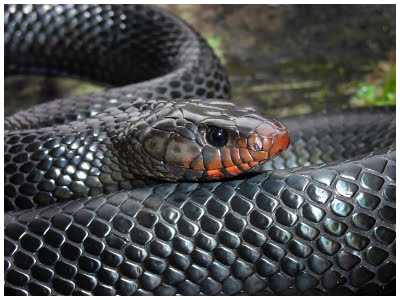
\includegraphics[height = 5cm]{media/indigo-snake-walton-outdoors.jpg}
        \end{figure}
    \end{column}
\end{columns}   
\end{frame}

\begin{frame}{Folt et al. (2019) - Extinction Models}
\begin{columns}
    \begin{column}[c]{5cm}
        \begin{itemize}
            \item Modeled the probabilty of extinctions for reintroduction efforts
            \item Found that 30 sub-adults over 10 years is the best case scenario
            \item Lacks any population genetics parameters
        \end{itemize}
    \end{column}

    \begin{column}[t]{8cm}
        \begin{figure}
            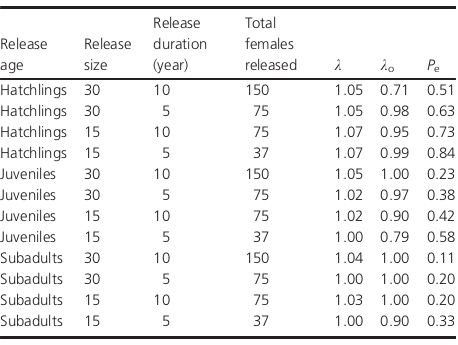
\includegraphics[height = 7cm]{media/folt-probabilities.png}
        \endP{figure}
    \end{column}
\end{columns}
\end{frame}

% \begin{frame}{Spring and Summer 2021}
  
%   \begin{itemize}
%   \item Classes
%   \begin{itemize}
%     \item Scripting for Biologists
%   \end{itemize}
%     \item GRA Support 
%     \begin{itemize}
%       \item Worked in the lab with two undergraduate students inventorying and quantifying extracts
%       \item Tested extraction protocols for shed skins from OCIC and Wild
%       \item Wrote Two Grants with JRO and BAC
%       \begin{itemize}
%         \item Section 6 to Alabama
%         \item Competitive State Wildlife Grant (CSWG) for Alabama
%       \end{itemize}
%     \end{itemize}

%   \end{itemize}
% \end{frame}

% \begin{frame}{Fall 2021}
%   \begin{itemize}
%     \item GTA Support
%     \begin{itemize}
%       \item Teaching A\&P I and II 
%     \end{itemize}
%     \item Classes
%     \begin{itemize}
%       \item Practical Evolution 
%       \item Agent Based Modelling 
%     \end{itemize}
%     \item Lab Work
%     \begin{itemize}
%       \item Down to one undergraduate
%       \item Finished concentrating Indigo extractions
%       \item About to begin RADSeq library prep and send sample for WGS
%       \item Began quantifying \textit{Laticauda} and \textit{Pachydactylus} extracts
%     \end{itemize}
%     \item Grants
%     \begin{itemize}
%       \item New Section 6 grant through Florida with JRO
%     \end{itemize}
    
%   \end{itemize}
% \end{frame}

% \section[New Projects]{New Projects}

% \begin{frame}{\textit{Laticauda} Project Synopsis}
%   \begin{itemize}
%     \item Extending my thesis work on sea kraits
%     \item Indo-Pacific marine adapted snake species
%     \item \textit{Laticauda} phylogenetics using RADSeq data
%     \item Population genetics of \textit{L. colubrina} species group 
%     \item Re-analyze genomic data from Kishida et al. (2021)
%   \end{itemize}
% \end{frame}


% \begin{frame}{\textit{Laticauda} Project Synopsis}
%   \begin{columns}[c]
%     % \begin{column}[c]{5cm}
%     %   \begin{itemize}
%     %     \item Extending my thesis work
%     %     \item \textit{Laticauda} phylogenetics using RADSeq data
%     %     \item Population genetics of \textit{L. colubrina} species group 
%     %     \item Re-analyze genomic data from Kishida et al. (2021)
%     %   \end{itemize}
%     % \end{column}
    
%     \begin{column}[t]{20cm}
%       \includegraphics[height = 8cm]{media/colubrina-02-discussion.png}
%     \end{column}
%   \end{columns}
% \end{frame}

% \begin{frame}{\textit{Laticauda} Project Synopsis}
%   \begin{columns}[c]
%     \begin{column}[c]{5cm}
%       \begin{itemize}
%         \item Re-analyze genomic data from Kishida et al. (2021)
%         \begin{itemize}
%           \item They suggest admixture between all species
%           \item Approx. 4 MYA origin for genus
%         \end{itemize}
%       \end{itemize}
%     \end{column}
    
%     \begin{column}[c]{10cm}
%       \begin{figure}
%         \hspace{-2.5cm}
%         \includegraphics[height = 4cm]{media/kishida-time-tree.png}

%         \caption{\parbox{4cm}{Weird time-calibrated tree from Kishida et al. (2021)}}
%       \end{figure}

%     \end{column}
%   \end{columns}
% \end{frame}


% \begin{frame}{\textit{Pachydactylus} Project Synopsis}
%   \begin{columns}[c]
%     \begin{column}[c]{5cm}
%       \begin{itemize}
%         \item Southern African gecko genus 
%         \item Potential ongoing hybridization between \textit{P. carinatus}[\textbf{Red}] and \textit{P. montanus}[\textbf{Blue}]
%         \item Writing sanger data manuscripts
%       \end{itemize}
%     \end{column}

%     \begin{column}[c]{10cm}
%       \includegraphics[height = 4.5 cm]{media/pachydactylus.jpg}
%     \end{column}
%   \end{columns}
% \end{frame}


% \begin{frame}{\textit{Pachydactylus} Project Synopsis}
%   \begin{columns}[c]
%     \begin{column}[c]{7cm}
%       \begin{figure}
%       \hspace*{-0.4cm}
%       \includegraphics[height = 7 cm]{media/pachydactylus-map.pdf}
%       \vspace{-1cm}
%       \caption{\parbox[t]{3cm}{Red - \textit{P. carinatus}, Blue - \textit{P. montanus}}}
%       \end{figure}
%     \end{column}

%     \begin{column}[c]{8cm}
%       \hspace*{-1.0cm}
%       \includegraphics[height=9cm]{media/stacey-all-data.pdf} 
%     \end{column}
%   \end{columns}
% \end{frame}


% \section[Dissertation Status]{Dissertation Update}

% \begin{frame}[fragile]{Indigo Snake Sequencing Efforts}
% \begin{itemize}
%   \item Approx. 300 individuals concentrated and ready for library prep
%   \begin{itemize}
%     \item About 50 breeders from the OCIC
%     \item About 250 Wild Individuals
%   \end{itemize}
%   \item Additional 400 individuals available for future sequencing
%   \item Whole Genome Sequence using PacBio Sequel II Platform
% \end{itemize}
% \end{frame}

% \begin{frame}{Chapter 1: Genus Phylogeography}
%   \begin{itemize}

%     \item Requesting tissue samples of other species in \textit{Drymarchon}
%     \item This will be the first phylogeny for the group
%     \item Taxon sampling will be an issue
%     \begin{itemize}
%       \item Five Species
%       \item Maybe 60 samples available - mostly \textit{D. corais}
%       \item Missing two South American taxa
%     \end{itemize}

%   \end{itemize}
% \end{frame}

% \begin{frame}{Chapter 2: Population Genomics of Wild Populations}
%   \begin{columns}[t]{}
%     \begin{column}[T]{5cm}
%       \begin{itemize}
%         \item Use the RADSeq data to assess gene flow between Populations
%         \item Look for differentiation between geographically isolated Populations
%         \begin{itemize}
%           \item Western Florida Islands
%           \item Southern Georgia
%         \end{itemize}
%       \end{itemize}
%     \end{column}
%     \begin{column}[T]{10cm}
%       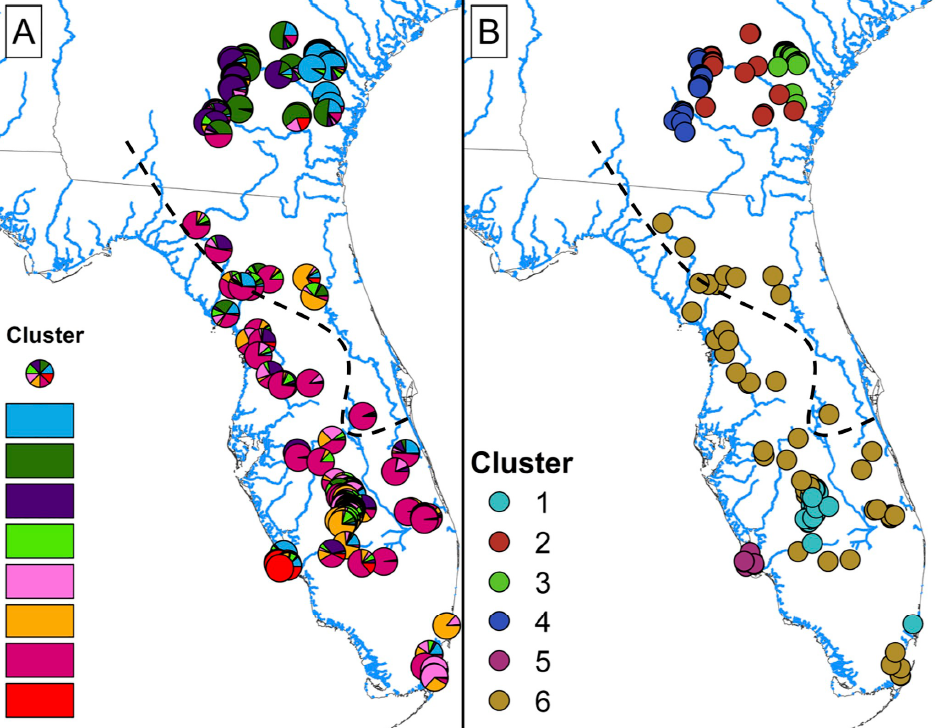
\includegraphics[height = 5.7cm]{media/indigo-snakes-genetic-clusters.PNG}
%     \end{column}
%   \end{columns}
% \end{frame}

% \begin{frame}{Chapter 3: Pedigree and Genetic Diversity of OCIC Colony}
%   \begin{columns}[T]{}
%     \begin{column}[t]{6cm}
%       \begin{itemize}
%         \item Working with Dr. Bogan at OCIC to get shed skins for all indigos
%         \item Use RADSeq data to estimate pedigree and genetic diveristy of the OCIC colony 
%         \begin{itemize}
%           \item Determine if sperm retention is occurring in the OCIC
%         \end{itemize}
%         \item New Section 6 grant will focus on this work
%       \end{itemize}  
%     \end{column}
    
%     \begin{column}{10cm}
%     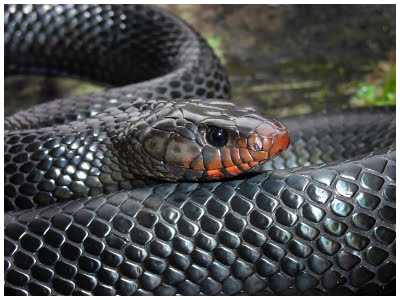
\includegraphics[height = 5cm]{media/indigo-snake-walton-outdoors.jpg}
%     \end{column}
%   \end{columns}
% \end{frame}

% \begin{frame}{Chapter 4: Forward in Time Simulations}
% \begin{columns}[c]
%   \begin{column}{6cm}
%     \begin{itemize}
%       \item Model reintroduction population viabilities using SLiM
%       \begin{itemize}
%         \item Build on the work of Folt et al. (2019)
%       \end{itemize}
%       \item Ongoing project in Practical Evolution
%       \item Vary sex ratios, yearly cohort size, length of introduction, source populations
%       \item Explore impacts on genetic diversity, adaptiveness, population growth
%     \end{itemize}
%   \end{column}
  
%   \begin{column}{10cm}
%     \hspace*{1cm}
%     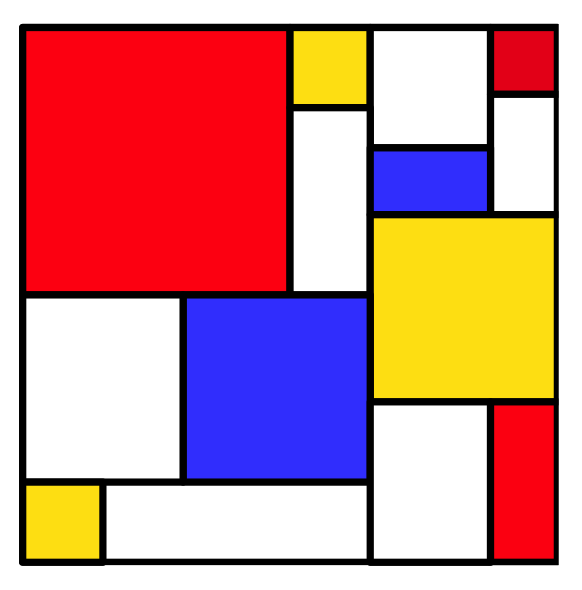
\includegraphics[height = 5cm]{media/slim-logo.png}
%   \end{column}
% \end{columns}
% \end{frame}

% \section[Year Goals]{Future Directions}

% \begin{frame}{Spring and Summer 2022}
%   \begin{itemize}
%     \item GRA support
%     \begin{itemize}
%       \item Finish getting RADSeq data for dissertation 
%       \item Get RADSeq data for \textit{Pachydactylus} and \textit{Laticauda}
%       \item Working with two undergraduates
%     \end{itemize}
%     \item Personal Goals
%     \begin{itemize}
%       \item Complete proposal by Spring Break
%       \begin{itemize}
%         \item Primarily pull from written grants
%       \end{itemize}
%       \item Do written exam by the end of the Spring semester
%       \item Proposal seminar during the summer
%       \begin{itemize}
%         \item Be able to incorporate preliminary data
%       \end{itemize}
%     \end{itemize}
%     \item Classes
%     \begin{itemize}
%       \item No
%     \end{itemize}
%   \end{itemize}

% \end{frame}

% \begin{frame}{Questions?}
%   \begin{center}
%     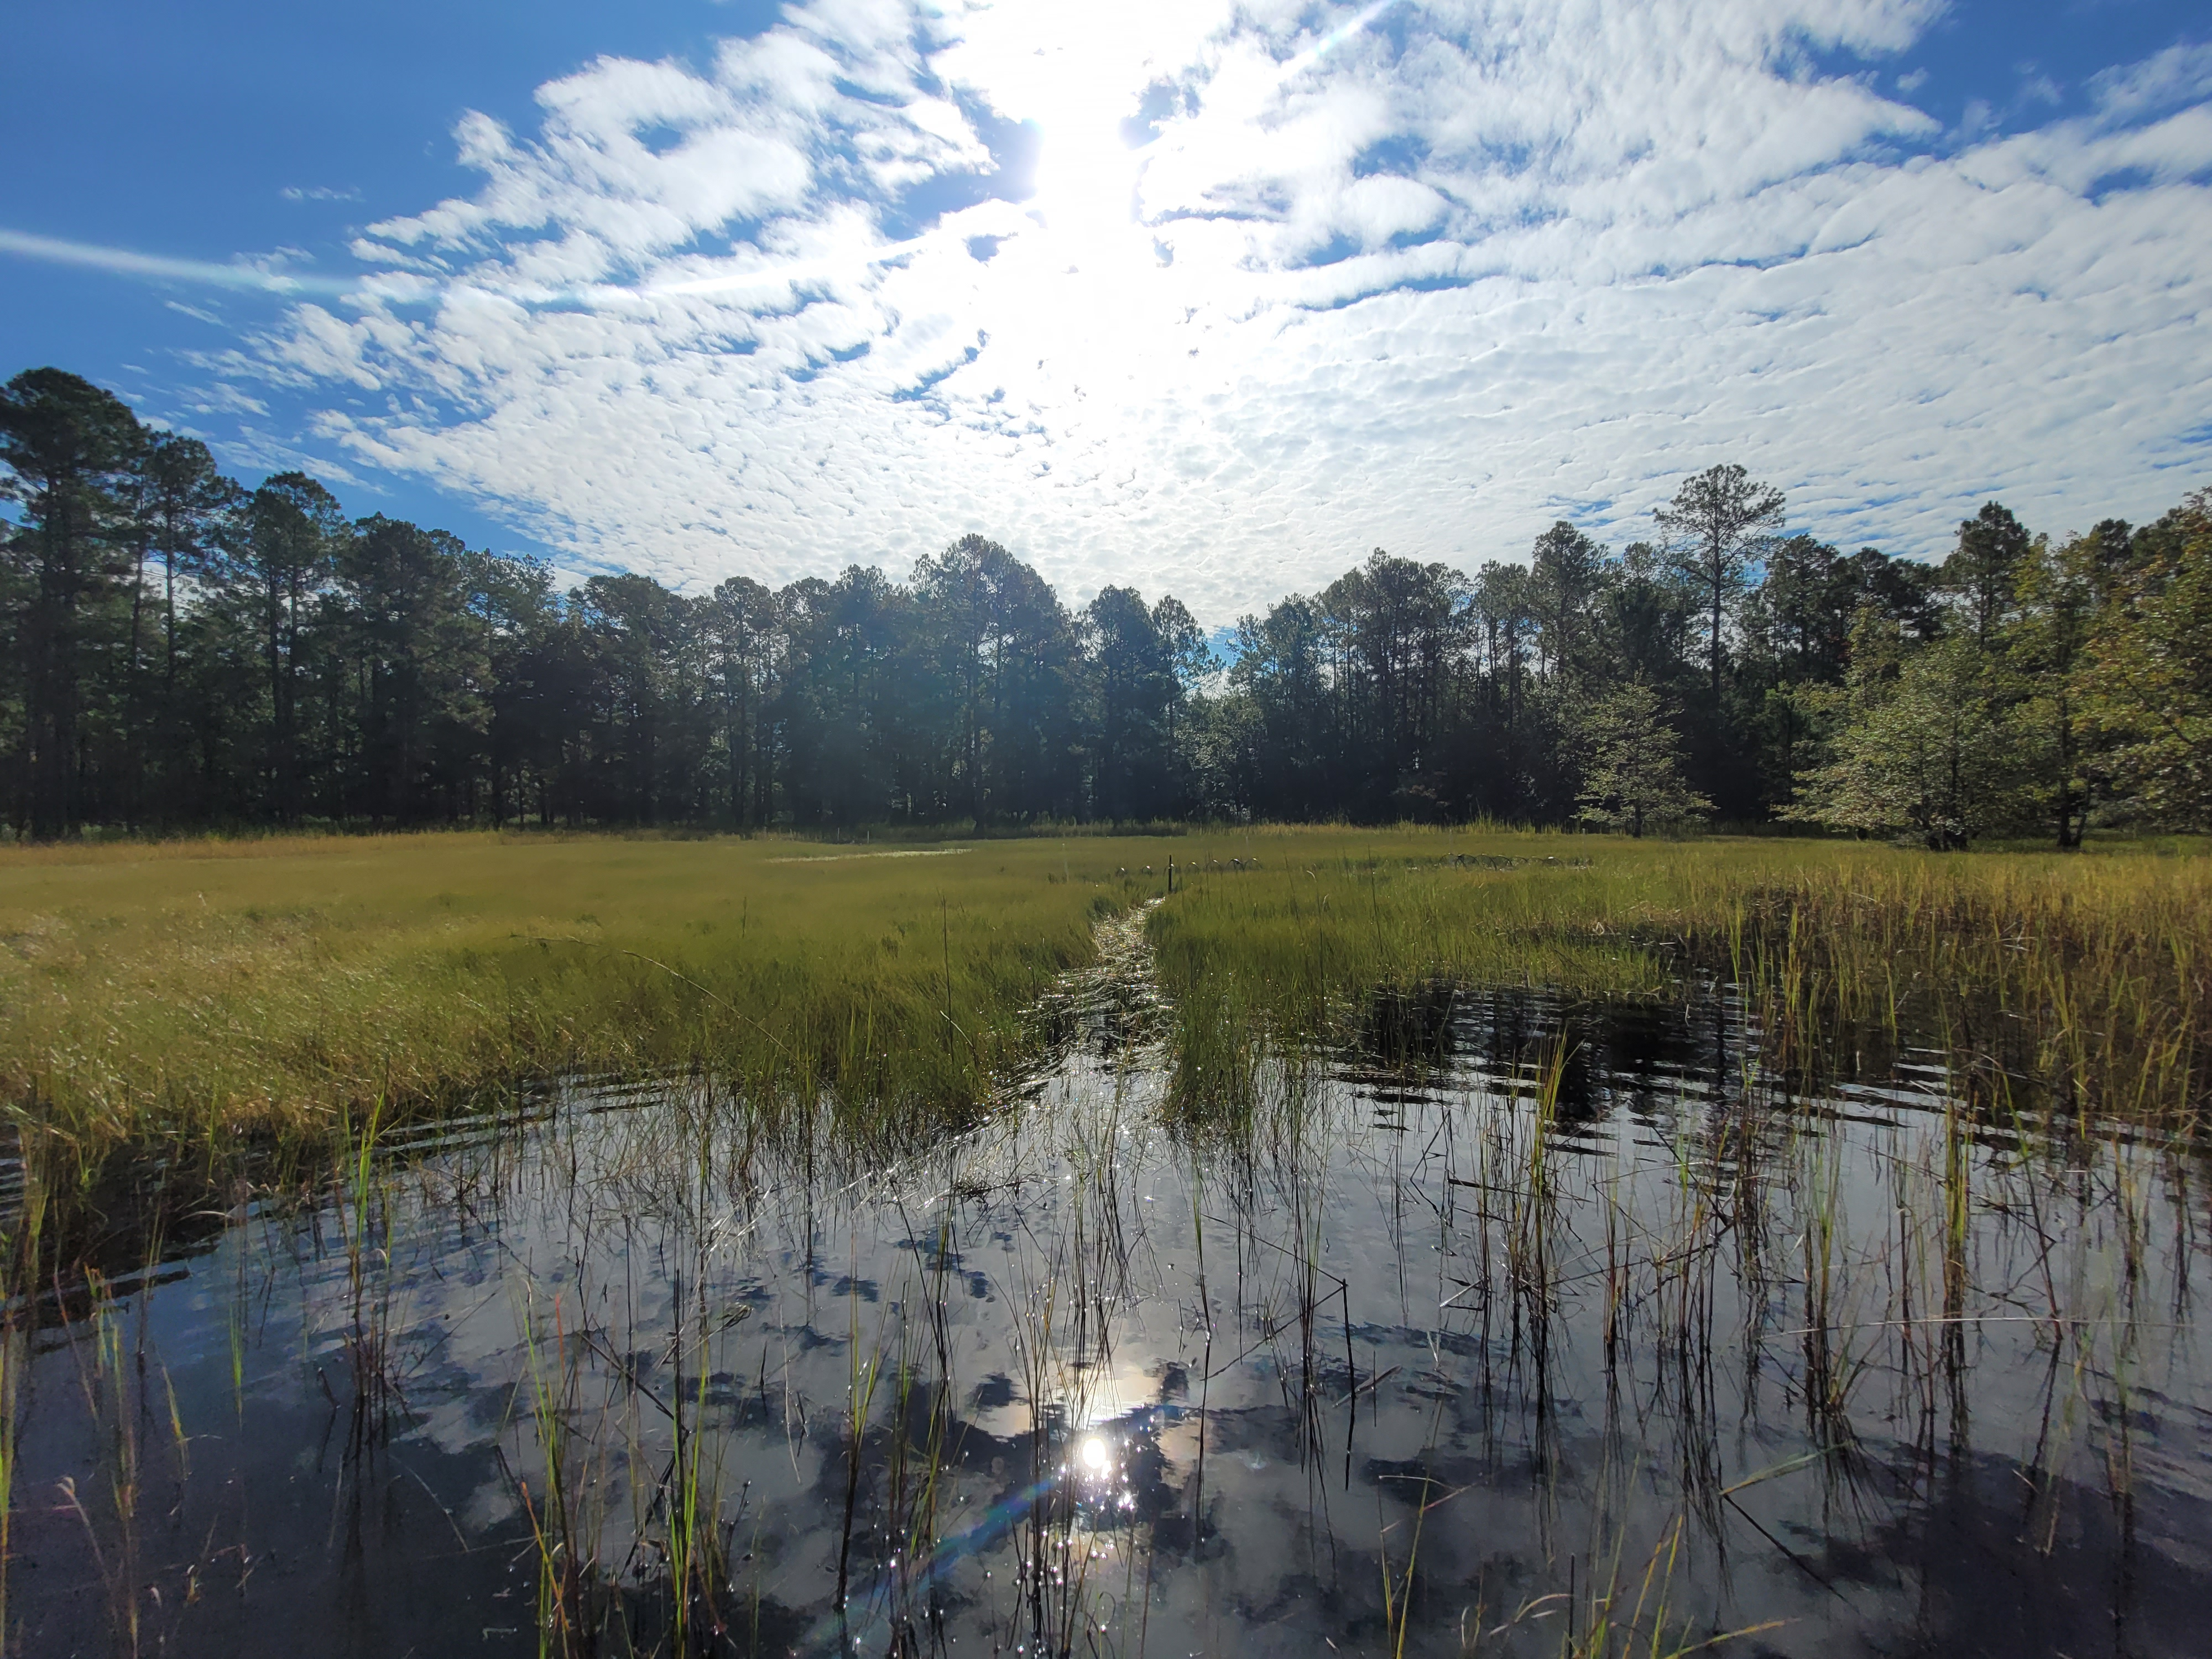
\includegraphics[height = 7.5cm]{media/conecuh-pond.jpg}    
%   \end{center}

% \end{frame}



\end{document}
